\documentclass[11pt,a4paper]{article}

% ── Packages ──────────────────────────────────────────────────────────
\usepackage[margin=1in]{geometry}
\usepackage{amsmath,amssymb,amsthm}
\usepackage{bm}
\usepackage{booktabs}
\usepackage{graphicx}
\usepackage{hyperref}
\usepackage{cleveref}
\usepackage{algorithm}
\usepackage{algpseudocode}
\usepackage{natbib}
\usepackage{xcolor}

\hypersetup{
    colorlinks=true,
    linkcolor=blue!70!black,
    citecolor=green!50!black,
    urlcolor=blue!60!black,
}

% ── Math shortcuts ────────────────────────────────────────────────────
\newcommand{\R}{\mathbb{R}}
\newcommand{\vp}{\varphi}
\newcommand{\xwec}{\bm{x}_{\mathrm{wec}}}
\newcommand{\xopt}{\bm{x}_{\mathrm{opt}}}
\newcommand{\bh}{\bm{h}}
\newcommand{\blam}{\bm{\lambda}}
\newcommand{\bmu}{\bm{\mu}}
\newcommand{\btheta}{\bm{\theta}}
\newcommand{\pd}[2]{\frac{\partial #1}{\partial #2}}
\newcommand{\dd}[2]{\frac{d #1}{d #2}}

\title{Gradient-Based Hull Shape Optimization for \\
       Wave Energy Converters via Hybrid \\
       Analytical--Finite-Difference Sensitivities}

\author{Kapil Khanal}
\date{\today}

\begin{document}
\maketitle

% ══════════════════════════════════════════════════════════════════════
\begin{abstract}
We present a gradient-based framework for optimizing the hull geometry
of a wave energy converter (WEC) to maximize electrical power output.
The approach exploits a bilevel structure: an inner nonlinear program
(NLP) solved by IPOPT determines the optimal power take-off (PTO)
control for a given hull shape, while an outer optimizer adjusts the
hull shape parameters.  The key contribution is a \emph{hybrid gradient}
that combines (i)~an \emph{analytical} Fiacco post-optimality sensitivity
for the derivative of optimal power with respect to boundary element
method (BEM) hydrodynamic coefficients, with (ii)~\emph{finite differences}
through the BEM solver (Capytaine) for the derivative of hydrodynamic
coefficients with respect to hull shape parameters.  The chain rule
links these two components, yielding an accurate gradient at a fraction
of the cost of full finite-difference optimization.  We demonstrate the
method on the AquaHarmonics device, optimizing the main cylinder radius
and draft under a regular wave condition.
\end{abstract}

\tableofcontents
\newpage

% ══════════════════════════════════════════════════════════════════════
\section{Introduction}
\label{sec:intro}

The design of wave energy converters involves coupled decisions about
hull geometry and control strategy.  Hull shape determines the
hydrodynamic response---added mass, radiation damping, excitation
forces---which in turn governs the achievable power under optimal
control.  Traditional shape optimization relies on derivative-free
methods (e.g., genetic algorithms, Nelder--Mead) because the
shape-to-power pipeline involves non-differentiable components:
mesh generation, BEM solvers, and NLP solvers.

We propose a hybrid approach that renders this pipeline
\emph{partially differentiable}.  The expensive NLP solve is handled
analytically via the Fiacco post-optimality sensitivity theorem
(also known as the envelope theorem), while the BEM solver is
treated as a black box and differentiated via finite differences.
This reduces the cost of each gradient evaluation from
$\mathcal{O}(n_{\text{shape}})$ full NLP solves to
$\mathcal{O}(n_{\text{shape}})$ BEM solves plus a single NLP solve,
often an order-of-magnitude speedup.


% ══════════════════════════════════════════════════════════════════════
\section{WEC Dynamics and Pseudo-Spectral Formulation}
\label{sec:dynamics}

\subsection{Equation of Motion}

The dynamics of a floating body in waves are governed by the
Cummins equation.  In the frequency domain, for a single degree of
freedom (heave), the equation of motion is
\begin{equation}
\label{eq:eom_freq}
    -\omega^2 \bigl[M + A(\omega)\bigr]\hat{X}(\omega)
    + j\omega \bigl[B(\omega) + B_f\bigr]\hat{X}(\omega)
    + K\,\hat{X}(\omega)
    = \hat{F}_{\mathrm{exc}}(\omega) + \hat{F}_{\mathrm{PTO}}(\omega),
\end{equation}
where:
\begin{itemize}
    \item $M$ is the rigid-body inertia matrix,
    \item $A(\omega)$ is the frequency-dependent added mass,
    \item $B(\omega)$ is the radiation damping,
    \item $B_f$ is linear friction (supplementary damping),
    \item $K$ is the hydrostatic stiffness,
    \item $\hat{F}_{\mathrm{exc}}(\omega)
          = \hat{F}_{\mathrm{FK}}(\omega) + \hat{F}_{\mathrm{diff}}(\omega)$
          is the wave excitation force
          (Froude--Krylov plus diffraction), and
    \item $\hat{F}_{\mathrm{PTO}}(\omega)$ is the PTO force
          (a decision variable in the control optimization).
\end{itemize}

\subsection{Pseudo-Spectral Discretization}

WecOptTool uses a pseudo-spectral method that represents the WEC
state~$x(t)$ via a truncated Fourier series.  Let $f_1$ be the
fundamental frequency and $N_f$ the number of harmonics.  The state
vector is
\begin{equation}
    \xwec = \bigl[\mathrm{Re}(\hat{X}_1),\;\mathrm{Im}(\hat{X}_1),\;
    \ldots,\;\mathrm{Re}(\hat{X}_{N_f})\bigr]^\top
    \in \R^{2N_f - 1},
\end{equation}
where the imaginary part of the highest frequency is excluded
(Nyquist constraint).  Derivatives and time-domain evaluations are
computed via the time matrix~$\bm{T}$ and derivative
matrix~$\bm{D}$:
\begin{equation}
    x(t_k) = \bm{T}\,\xwec, \qquad
    \dot{x}(t_k) = \bm{T}\bm{D}\,\xwec.
\end{equation}

The BEM-dependent forces in the time domain are:
\begin{align}
    \bm{f}_{\mathrm{rad}} &= \bm{T}\,\bm{Z}_{\mathrm{rad}}\,\xwec,
    &\bm{Z}_{\mathrm{rad}} &= \text{blkdiag}\bigl(
        j\omega_k B(\omega_k) - \omega_k^2 A(\omega_k)\bigr),
    \label{eq:f_rad} \\
    \bm{f}_{\mathrm{hs}} &= \bm{T}\,\bm{Z}_{\mathrm{hs}}\,\xwec,
    &\bm{Z}_{\mathrm{hs}} &= \text{blkdiag}(K),
    \label{eq:f_hs} \\
    \bm{f}_{\mathrm{fric}} &= \bm{T}\,\bm{Z}_{\mathrm{fric}}\,\xwec,
    &\bm{Z}_{\mathrm{fric}} &= \text{blkdiag}(j\omega_k B_f),
    \label{eq:f_fric} \\
    \bm{f}_{\mathrm{exc}} &= \bm{T}\,\mathrm{c2r}\Bigl(
        \textstyle\sum_\theta \hat{\eta}(\omega,\theta)\,
        X_{\mathrm{exc}}(\omega,\theta)\Bigr),
    \label{eq:f_exc}
\end{align}
where $\text{blkdiag}(\cdot)$ denotes the real block-diagonal
representation of complex MIMO transfer matrices (mapping Fourier
coefficients to Fourier coefficients), and $\mathrm{c2r}(\cdot)$
converts complex Fourier coefficients to the real state
representation.

\subsection{Dynamics Residual}

The dynamics equality constraint is the residual
\begin{equation}
\label{eq:residual}
    r(\xwec, \xopt; \bh)
    = \underbrace{-\omega^2 M\,\xwec}_{\text{inertia}}
    - \underbrace{\bm{f}_{\mathrm{rad}}(\bh)}_{\text{radiation}}
    - \underbrace{\bm{f}_{\mathrm{hs}}(\bh)}_{\text{hydrostatics}}
    - \underbrace{\bm{f}_{\mathrm{fric}}(\bh)}_{\text{friction}}
    - \underbrace{\bm{f}_{\mathrm{exc}}(\bh)}_{\text{excitation}}
    - \underbrace{\bm{f}_{\mathrm{add}}(\xwec, \xopt)}_{\text{PTO, buoyancy, \ldots}}
    = \bm{0},
\end{equation}
where $\bh = (A, B, K, B_f, F_{\mathrm{FK}}, F_{\mathrm{diff}}, M)$
collects all BEM-dependent hydrodynamic parameters, and
$\bm{f}_{\mathrm{add}}$ includes forces that do \emph{not} depend
on~$\bh$ (PTO, buoyancy, gravity, mooring).


% ══════════════════════════════════════════════════════════════════════
\section{Bilevel Optimization Problem}
\label{sec:bilevel}

\subsection{Inner Problem: Optimal WEC Control}

For a fixed hull shape (and hence fixed BEM coefficients~$\bh$), the
optimal control problem is the NLP:
\begin{equation}
\label{eq:inner}
\boxed{
\begin{aligned}
    \vp^*(\bh) = \min_{\xwec, \xopt} \quad
        & f(\xwec, \xopt) \\
    \text{subject to} \quad
        & r(\xwec, \xopt; \bh) = \bm{0}
            && \text{(dynamics, } \blam \text{)} \\
        & g_i(\xwec, \xopt) \ge \bm{0}, \quad i=1,\ldots,m
            && \text{(inequality constraints, } \bmu_i \text{)}
\end{aligned}
}
\end{equation}
where $f$ is the objective (e.g., average electrical power from the PTO),
$\blam$ and~$\bmu_i$ are the Lagrange multipliers returned by IPOPT.

For the AquaHarmonics device, the inequality constraints include:
\begin{enumerate}
    \item Peak PTO torque limit: $\tau_{\max} - |\tau(t)| \ge 0$
    \item Maximum rotational speed: $\dot{\phi}_{\max} - |\dot{\phi}(t)| \ge 0$
    \item Maximum mechanical power: $P_{\max} - |P_{\mathrm{mech}}(t)| \ge 0$
    \item Minimum mooring line tension: $T(t) + T_{\min} \ge 0$
    \item Zero mean heave position: $\bar{x} = 0$ (equality)
\end{enumerate}

\subsection{Outer Problem: Hull Shape Optimization}

The outer problem adjusts the hull shape parameters
$\btheta \in \R^{n_\theta}$ to maximize the optimal power:
\begin{equation}
\label{eq:outer}
    \max_{\btheta} \quad \vp^*\bigl(\bh(\btheta)\bigr)
    \qquad \text{subject to} \qquad
    \btheta^{\min} \le \btheta \le \btheta^{\max}.
\end{equation}

For the AquaHarmonics device, we parameterize the hull by:
\begin{itemize}
    \item $\theta_1 = r_1$: radius of the main (upper) cylinder [m],
          $r_1 \in [0.5, 2.5]$
    \item $\theta_2 = T_1$: draft of the main cylinder [m],
          $T_1 \in [0.5, 3.0]$
\end{itemize}
with default values $r_1 = 1.085$\,m and $T_1 = 1.5$\,m.  The
remaining dimensions ($T_2$, $T_3$, $r_2$, $r_3$) are held fixed.


% ══════════════════════════════════════════════════════════════════════
\section{Gradient Computation}
\label{sec:gradient}

The total derivative of optimal power with respect to shape is
\begin{equation}
\label{eq:chain_rule}
    \dd{\vp^*}{\theta_j}
    = \sum_{i} \dd{\vp^*}{h_i} \cdot \dd{h_i}{\theta_j},
    \qquad j = 1, \ldots, n_\theta.
\end{equation}
We compute the two factors using different strategies.

\subsection{Analytical: Fiacco Post-Optimality Sensitivity}
\label{sec:fiacco}

The Fiacco sensitivity theorem~\citep{fiacco1976sensitivity} (also
known as the envelope theorem) states that at an optimal solution
$(\xwec^*, \xopt^*)$ with Lagrange multipliers~$\blam^*$,
$\bmu_i^*$, the total derivative of the optimal objective with
respect to a parameter~$h$ is:
\begin{equation}
\label{eq:fiacco_full}
    \dd{\vp^*}{h}
    = \pd{f}{h}\bigg|_{x^*}
    + {\blam^*}^\top \pd{r}{h}\bigg|_{x^*}
    + \sum_{i=1}^{m} {\bmu_i^*}^\top \pd{g_i}{h}\bigg|_{x^*}.
\end{equation}

For the AquaHarmonics device, several simplifications apply:
\begin{enumerate}
    \item The objective $f = \text{pto.average\_power}$ depends only on
          $(\xwec, \xopt)$ and not on~$\bh$ directly, so
          $\pd{f}{\bh} = \bm{0}$.
    \item The inequality constraints (torque, speed, power, tension)
          depend only on $(\xwec, \xopt)$ and not on~$\bh$, so
          $\pd{g_i}{\bh} = \bm{0}$ for all~$i$.
\end{enumerate}

Therefore, the Fiacco formula reduces to:
\begin{equation}
\label{eq:fiacco_reduced}
\boxed{
    \dd{\vp^*}{\bh}
    = {\blam^*}^\top \pd{r}{\bh}\bigg|_{(\xwec^*, \xopt^*)}
}
\end{equation}

\paragraph{Implementation via VJP.}
The vector-Jacobian product (VJP) ${\blam^*}^\top
\frac{\partial r}{\partial \bh}$ is computed efficiently using
reverse-mode automatic differentiation (JAX).  Define
\begin{equation}
    r_h(\bh) \;=\; r(\xwec^*, \xopt^*; \bh),
\end{equation}
where the WEC state is held fixed at the optimum.  The VJP is
\begin{equation}
    \dd{\vp^*}{\bh} = \text{vjp}(r_h, \bh)^\top \blam^* .
\end{equation}

The function $r_h$ is implemented as
\texttt{residual\_parametric}---a pure JAX function that recomputes
the BEM-dependent forces (radiation, hydrostatics, friction,
excitation) from the parameter arrays, without calling the original
force closures.  This makes $\partial r / \partial \bh$ available to
JAX's AD system.

\paragraph{Computational cost.}
A single VJP evaluation costs $\mathcal{O}(1)$ times the cost of
evaluating~$r$ itself, regardless of the number of BEM
parameters~$n_h$.  For the AquaHarmonics device with $n_h = 63$
real-valued entries, this is essentially instantaneous compared to
the IPOPT solve.

\subsection{Finite Differences: BEM Jacobian}
\label{sec:fd_bem}

Since Capytaine (the BEM solver) is not differentiable, we estimate
$\partial \bh / \partial \theta_j$ via central finite differences:
\begin{equation}
\label{eq:fd_bem}
    \dd{h_i}{\theta_j}
    \approx \frac{h_i(\btheta + \epsilon\,\bm{e}_j)
                - h_i(\btheta - \epsilon\,\bm{e}_j)}{2\epsilon},
\end{equation}
where $\epsilon = 10^{-3} \max(|\theta_j|, 0.1)$ and $\bm{e}_j$ is
the $j$-th standard basis vector.

\paragraph{Computational cost.}
Each shape parameter requires two BEM evaluations (forward and
backward perturbation).  For $n_\theta = 2$ shape parameters, this
is 4~BEM solves per gradient evaluation.  Crucially, these BEM
solves do \emph{not} require re-solving the IPOPT problem---only
the hydrodynamic coefficients are needed.

\subsection{Hybrid Gradient via Chain Rule}
\label{sec:hybrid}

Combining \cref{eq:fiacco_reduced,eq:fd_bem} into the chain
rule~\eqref{eq:chain_rule}:
\begin{equation}
\label{eq:hybrid}
\boxed{
    \dd{\vp^*}{\theta_j}
    = \sum_{i=1}^{n_h}
      \underbrace{\dd{\vp^*}{h_i}}_{\text{Fiacco (analytical)}}
      \cdot
      \underbrace{\dd{h_i}{\theta_j}}_{\text{FD (Capytaine)}}
}
\end{equation}

In practice, this inner product is computed as:
\begin{equation}
    \dd{\vp^*}{\theta_j}
    = \sum_{k \in \mathcal{P}}
      \mathrm{Re}\!\left\langle
        \dd{\vp^*}{\bh_k},\;
        \dd{\bh_k}{\theta_j}
      \right\rangle,
\end{equation}
where $\mathcal{P} = \{A, B, K, B_f, F_{\mathrm{FK}},
F_{\mathrm{diff}}, M\}$ and the inner product accounts for complex
parameters (Froude--Krylov and diffraction forces) via conjugation.

\subsection{Cost Comparison}
\label{sec:cost}

\Cref{tab:cost} compares the per-iteration cost of the hybrid
gradient with a naive finite-difference approach that re-solves the
full NLP for each shape perturbation.

\begin{table}[ht]
\centering
\caption{Computational cost per gradient evaluation
         ($n_\theta$~shape parameters).}
\label{tab:cost}
\begin{tabular}{lcc}
\toprule
\textbf{Component} & \textbf{Hybrid (ours)} & \textbf{Full FD} \\
\midrule
IPOPT solves    & 1                      & $2n_\theta + 1$ \\
BEM solves      & $2n_\theta + 1$        & $2n_\theta + 1$ \\
VJP evaluations & 1                      & 0 \\
\midrule
\textbf{Dominant cost} & \textbf{1 IPOPT} & $\bm{2n_\theta + 1}$ \textbf{IPOPT} \\
\bottomrule
\end{tabular}
\end{table}

For the AquaHarmonics device with $n_\theta = 2$, the hybrid method
requires 1~IPOPT solve versus 5~IPOPT solves for full FD---a
$5\times$ reduction in the most expensive component.  The advantage
grows linearly with~$n_\theta$.


% ══════════════════════════════════════════════════════════════════════
\section{Optimization Algorithm}
\label{sec:algorithm}

The complete shape optimization procedure is given in
\Cref{alg:shape_opt}.

\begin{algorithm}[ht]
\caption{Gradient-based hull shape optimization}
\label{alg:shape_opt}
\begin{algorithmic}[1]
\Require Initial shape $\btheta^{(0)}$, bounds
         $[\btheta^{\min}, \btheta^{\max}]$, FD step $\epsilon$
\Ensure Optimized shape $\btheta^*$
\State $\bm{x}^{(0)}_{\mathrm{warm}} \gets \texttt{None}$
\For{$k = 0, 1, 2, \ldots$ until convergence}
    \State \textbf{--- Shape-to-Power Pipeline ---}
    \State $\bh^{(k)} \gets \texttt{Capytaine}(\btheta^{(k)})$
        \Comment{Mesh + BEM}
    \State $(\xwec^*, \xopt^*, \blam^*) \gets
        \texttt{IPOPT}(\bh^{(k)}, \bm{x}^{(k)}_{\mathrm{warm}})$
        \Comment{Inner NLP solve}
    \State $\vp^{(k)} \gets f(\xwec^*, \xopt^*)$
    \State $\bm{x}^{(k+1)}_{\mathrm{warm}} \gets (\xwec^*, \xopt^*)$
        \Comment{Warm-start for next iteration}
    \State \textbf{--- Hybrid Gradient ---}
    \State $\dd{\vp^*}{\bh} \gets
        {\blam^*}^\top \pd{r}{\bh}\big|_{x^*}$
        \Comment{Fiacco VJP (analytical)}
    \For{$j = 1, \ldots, n_\theta$}
        \State $\bh^+ \gets \texttt{Capytaine}(\btheta^{(k)}
            + \epsilon\,\bm{e}_j)$
        \State $\bh^- \gets \texttt{Capytaine}(\btheta^{(k)}
            - \epsilon\,\bm{e}_j)$
        \State $\dd{\vp^*}{\theta_j} \gets
            \sum_i \dd{\vp^*}{h_i}
            \cdot \frac{h_i^+ - h_i^-}{2\epsilon}$
            \Comment{Chain rule}
    \EndFor
    \State \textbf{--- Outer Update ---}
    \State $\btheta^{(k+1)} \gets
        \texttt{L-BFGS-B}\!\left(\btheta^{(k)},\;
        -\nabla_\theta \vp^*,\;
        [\btheta^{\min}, \btheta^{\max}]\right)$
\EndFor
\end{algorithmic}
\end{algorithm}

Key implementation details:
\begin{itemize}
    \item \textbf{Warm-starting}: the IPOPT solver is warm-started
          from the previous iteration's solution, greatly reducing
          convergence time as shape changes are typically small
          between iterations.
    \item \textbf{Sign convention}: we minimize $-\vp^*$ (negative
          power) since \texttt{scipy.optimize.minimize} performs
          minimization.
    \item \textbf{Bound constraints}: the L-BFGS-B algorithm
          natively handles the box constraints on~$\btheta$.
\end{itemize}


% ══════════════════════════════════════════════════════════════════════
\section{Application: AquaHarmonics Device}
\label{sec:application}

\subsection{Device Description}

The AquaHarmonics WEC is a heave-mode point absorber with a
complex drive train including:
\begin{itemize}
    \item A multi-stage gear system (gear ratios $R_{21}$, $R_{45}$,
          $R_{67}$)
    \item A pneumatic air spring
    \item A generator with Joule heating losses:
          $P_{\mathrm{loss}} = R_w (T_e / k_T)^2$
          where $R_w = 0.4\;\Omega$ and $k_T = 1.5\;\mathrm{Nm/A}$
\end{itemize}

The hull geometry consists of an upper cylinder (radius~$r_1$,
draft~$T_1$), a conical frustum transition (height~$T_2$), and a
lower tube (height~$T_3$, outer radius~$r_2$, inner radius~$r_3$).

\subsection{Problem Setup}

\begin{itemize}
    \item \textbf{Wave conditions}: Regular wave,
          $A = 0.5$\,m, $f = 0.12$\,Hz, $\phi = 30^\circ$
    \item \textbf{Frequency resolution}: $f_1 = 0.12$\,Hz,
          $N_f = 10$ harmonics
    \item \textbf{Shape parameters}: $\btheta = (r_1, T_1)$
    \item \textbf{Fixed geometry}: $T_2 = 0.355$\,m,
          $T_3 = 7.25$\,m, $r_2 = 0.405$\,m, $r_3 = 0.355$\,m
    \item \textbf{Mass}: $m = 5000$\,kg (fixed)
    \item \textbf{Optimizer}: L-BFGS-B via
          \texttt{scipy.optimize.minimize}
\end{itemize}

\subsection{Baseline Sensitivity}

\Cref{fig:baseline} shows the Fiacco sensitivity
$\max_i |d\vp^*/dh_i|$ for each BEM parameter group at the default
hull shape.  This reveals which hydrodynamic coefficients the optimal
electrical power is most sensitive to, and motivates the choice of
shape parameters that most affect these coefficients.

\begin{figure}[ht]
\centering
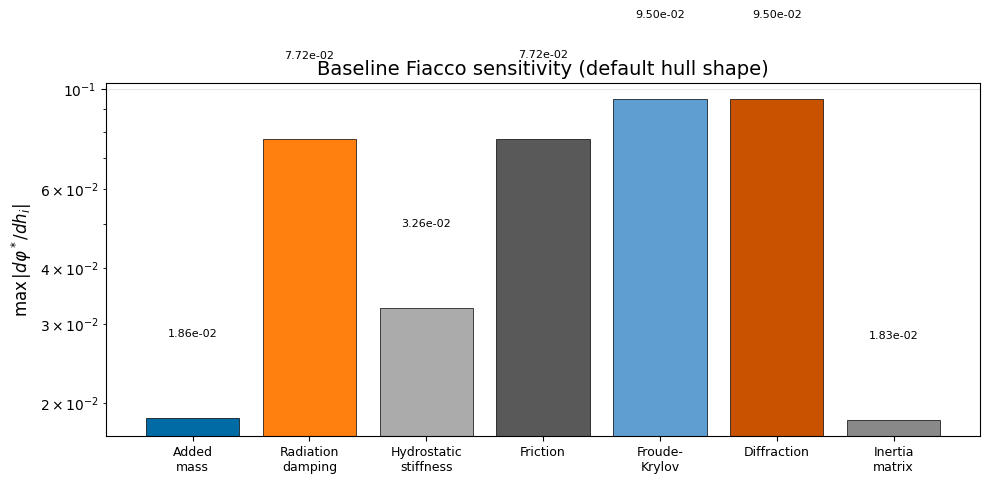
\includegraphics[width=0.85\textwidth]{fig_baseline_sensitivity.png}
\caption{Fiacco sensitivity of optimal electrical power to each BEM
         parameter group at the baseline hull shape
         ($r_1 = 1.085$\,m, $T_1 = 1.5$\,m).}
\label{fig:baseline}
\end{figure}

\subsection{Optimization Results}

The L-BFGS-B optimizer converges in a modest number of iterations.
\Cref{fig:convergence} shows the evolution of optimal power and the
two shape parameters across iterations.

\begin{figure}[ht]
\centering
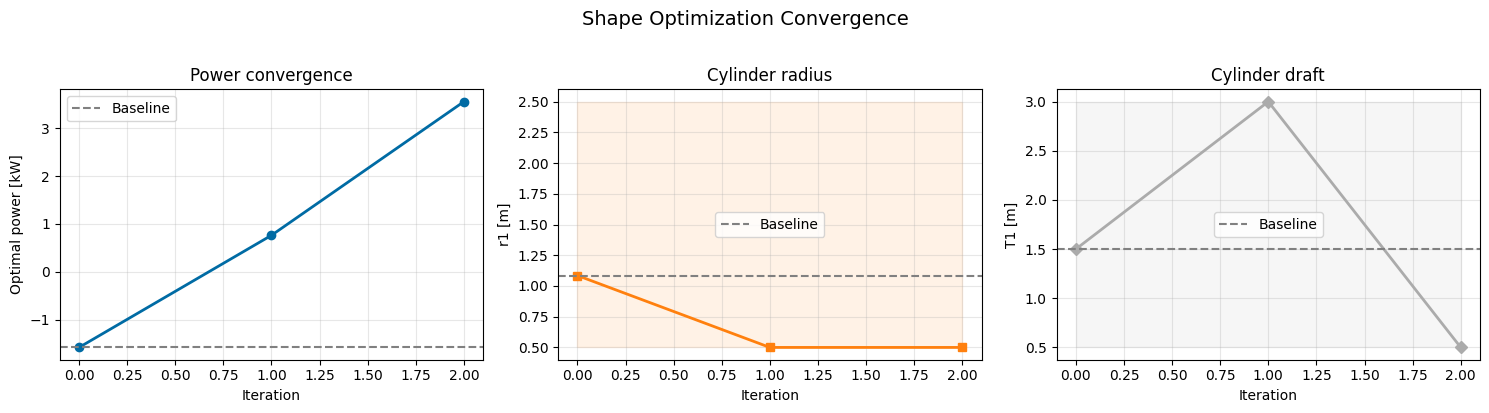
\includegraphics[width=\textwidth]{fig_convergence.png}
\caption{Convergence history of the shape optimization.
         Left: optimal electrical power vs.\ iteration.
         Center: cylinder radius~$r_1$.
         Right: cylinder draft~$T_1$.
         Dashed lines indicate baseline values; shaded regions
         indicate the feasible bounds.}
\label{fig:convergence}
\end{figure}

\Cref{fig:hull} compares the hull cross-sections of the baseline
and optimized designs.

\begin{figure}[ht]
\centering
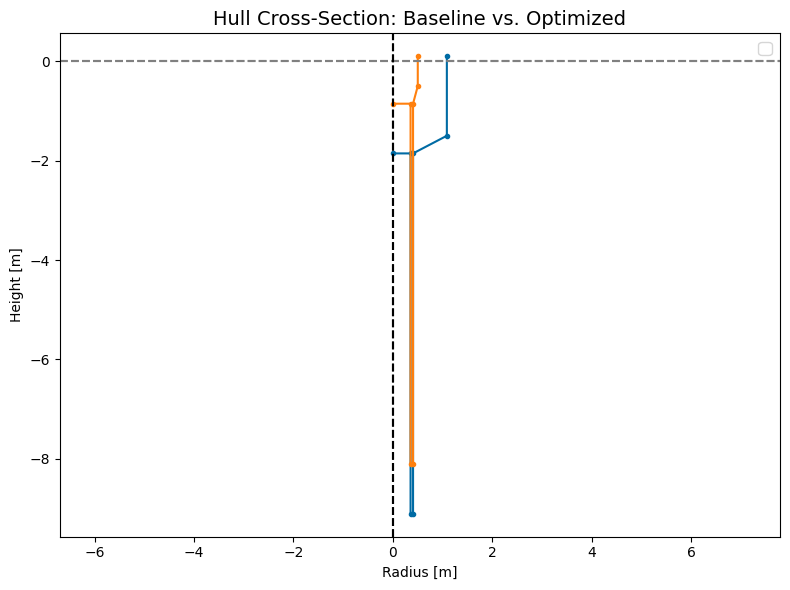
\includegraphics[width=0.65\textwidth]{fig_hull_comparison.png}
\caption{Hull cross-section comparison: baseline (blue) vs.\
         optimized (orange) AquaHarmonics geometry.}
\label{fig:hull}
\end{figure}

\Cref{fig:sensitivity_comparison} compares the Fiacco sensitivity
at the baseline and optimized shapes, revealing how the sensitivity
profile changes with hull geometry.

\begin{figure}[ht]
\centering
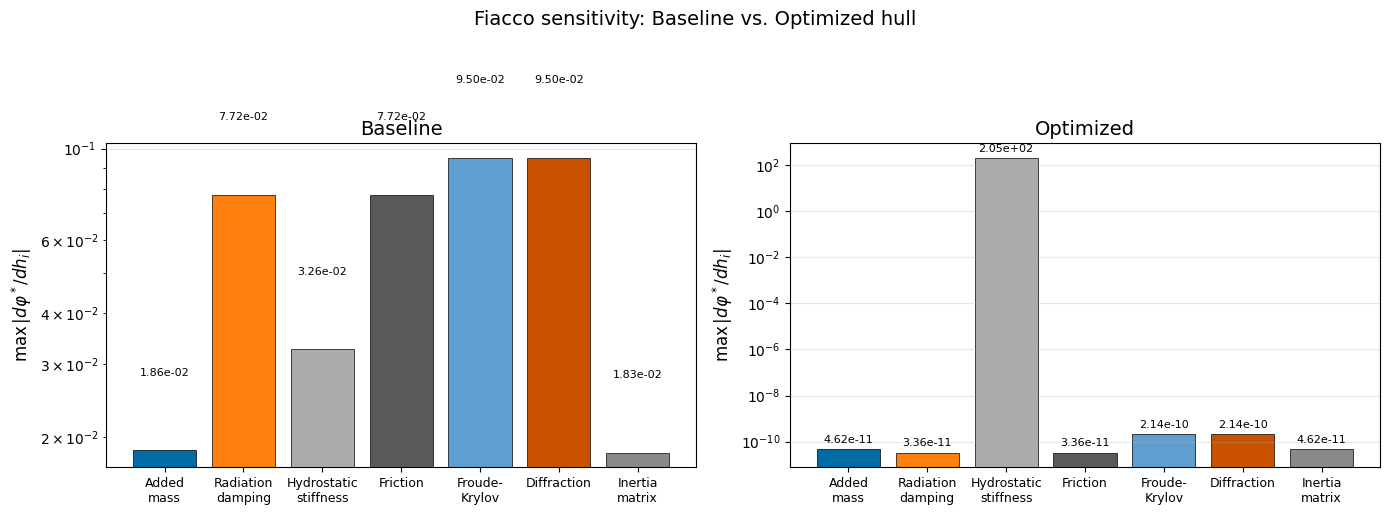
\includegraphics[width=\textwidth]{fig_sensitivity_comparison.png}
\caption{Fiacco sensitivity comparison between baseline and
         optimized hull shapes.  The sensitivity profile shifts as
         the optimizer adjusts the hull to maximize power.}
\label{fig:sensitivity_comparison}
\end{figure}


% ══════════════════════════════════════════════════════════════════════
\section{Software Implementation}
\label{sec:software}

The framework is implemented as extensions to
WecOptTool~\citep{wecopttool}, an open-source Python toolbox for
WEC design optimization.  The key modules are:

\begin{itemize}
    \item \texttt{wecopttool.solver\_ipopt}: Provides
          \texttt{WEC\_IPOPT}, a subclass of \texttt{WEC} that uses
          IPOPT (via \texttt{cyipopt}) and returns Lagrange
          multipliers.  Also provides \texttt{sensitivity()} for
          the Fiacco VJP and
          \texttt{make\_differentiable\_solver()} for a JAX-native
          interface with \texttt{jax.custom\_vjp}.
    \item \texttt{wecopttool.parametric}: Provides
          \texttt{residual\_parametric}---a pure JAX re-implementation
          of the BEM-dependent dynamics residual, compatible with
          \texttt{jax.vjp} and \texttt{jax.grad}.
    \item \texttt{wecopttool.sensitivity\_plots}: Reusable
          visualization utilities for sensitivity bar charts,
          per-frequency sensitivity plots, and analytical vs.\
          finite-difference comparison plots.
\end{itemize}

Dependencies include JAX (automatic differentiation), Capytaine
(BEM solver), IPOPT/cyipopt (NLP solver), and pygmsh/gmsh
(mesh generation).


% ══════════════════════════════════════════════════════════════════════
\section{Discussion}
\label{sec:discussion}

\subsection{Advantages}

\begin{enumerate}
    \item \textbf{Computational efficiency}: The hybrid gradient
          eliminates the need to re-solve the NLP for each finite
          difference perturbation.  The IPOPT solve (the dominant
          cost) is performed only once per outer iteration.
    \item \textbf{Gradient accuracy}: The Fiacco sensitivity is
          exact (to machine precision for the constraint term), while
          only the BEM Jacobian is approximated via finite differences.
    \item \textbf{Scalability}: The cost of the Fiacco VJP is
          independent of the number of BEM parameters ($n_h \approx 63$
          for the AquaHarmonics device).  The FD cost scales with
          $n_\theta$ (shape parameters), not~$n_h$.
    \item \textbf{Black-box BEM}: Capytaine is treated as a black
          box---no source-code modification or adjoint implementation
          is required.
\end{enumerate}

\subsection{Limitations and Future Work}

\begin{enumerate}
    \item \textbf{BEM finite differences}: The FD approximation of
          $\partial \bh / \partial \btheta$ introduces truncation error
          and requires careful step-size selection.  Differentiable
          BEM solvers (e.g., via AD through Capytaine or an adjoint
          method) would eliminate this entirely.
    \item \textbf{Single wave condition}: The current demonstration
          uses a single regular wave.  Extension to irregular sea
          states and multiple realizations is supported by the
          multi-realization feature in
          \texttt{make\_differentiable\_solver}.
    \item \textbf{Local optima}: The L-BFGS-B algorithm finds local
          optima.  Multi-start strategies or global optimization
          methods could be combined with the gradient information.
    \item \textbf{Additional shape parameters}: The current
          demonstration optimizes only $r_1$ and $T_1$.  The
          framework naturally extends to more parameters ($T_2$, $T_3$,
          $r_2$, $r_3$, or even free-form deformations).
\end{enumerate}


% ══════════════════════════════════════════════════════════════════════
\section{Conclusion}
\label{sec:conclusion}

We have presented a hybrid analytical--finite-difference framework for
gradient-based hull shape optimization of wave energy converters.  By
exploiting the Fiacco post-optimality sensitivity theorem, the method
avoids the dominant cost of re-solving the inner NLP for each shape
perturbation.  The framework is implemented as an extension to
WecOptTool and demonstrated on the AquaHarmonics device
(\cref{fig:hull}), where the optimizer converges in a modest number
of iterations (\cref{fig:convergence}) to an improved hull shape.

The key insight is that the bilevel structure of WEC design---hull
shape determines hydrodynamic coefficients, which determine optimal
control and power---can be efficiently exploited by computing exact
sensitivities through the inner optimization and approximating only
the non-differentiable BEM component via finite differences.


% ══════════════════════════════════════════════════════════════════════
\bibliographystyle{plainnat}
\begin{thebibliography}{9}

\bibitem[Fiacco(1976)]{fiacco1976sensitivity}
A.~V. Fiacco.
\newblock Sensitivity analysis for nonlinear programming using penalty methods.
\newblock \emph{Mathematical Programming}, 10(1):287--311, 1976.

\bibitem[Bacelli et~al.(2022)]{wecopttool}
G.~Bacelli, C.~B. Coe, et~al.
\newblock {WecOptTool}: An open-source toolbox for WEC design optimization.
\newblock Sandia National Laboratories, 2022.
\newblock \url{https://sandialabs.github.io/WecOptTool/}.

\bibitem[Ancellin and Dias(2019)]{capytaine}
A.~Ancellin and F.~Dias.
\newblock Capytaine: a {P}ython-based linear potential flow solver.
\newblock \emph{Journal of Open Source Software}, 4(36):1341, 2019.

\bibitem[W{\"a}chter and Biegler(2006)]{ipopt}
A.~W{\"a}chter and L.~T. Biegler.
\newblock On the implementation of an interior-point filter line-search
  algorithm for large-scale nonlinear programming.
\newblock \emph{Mathematical Programming}, 106(1):25--57, 2006.

\bibitem[Bradbury et~al.(2018)]{jax}
J.~Bradbury, R.~Frostig, et~al.
\newblock {JAX}: composable transformations of {P}ython+{N}um{P}y programs.
\newblock 2018.
\newblock \url{http://github.com/google/jax}.

\bibitem[Coe et~al.(2020)]{coe2020wec}
R.~G. Coe, G.~Bacelli, et~al.
\newblock A comparison of {WEC} control strategies.
\newblock Sandia National Laboratories, SAND2020-9087, 2020.

\end{thebibliography}


\end{document}
